\chapter{Simulación y Análisis de Sobrecarga}
\label{sec.c5:simulacion}

\section{Metodología experimental en LTspice}
\label{sec.c5:metodologia}

Para validar el circuito se utilizó los modelos SPICE del LM7812 y del TIP42C
proporcionado por los respectivos fabricantes.

Para evaluar el comportamiento de la fuente tanto en régimen normal de carga
como ante condiciones de sobrecarga y cortocircuito, se implementó en LTspice un
barrido paramétrico del resistor de carga ($R_L$) barriendo entre
$\SI{0.5}{\ohm}$ y $\SI{4.0}{\ohm}$ mediante un análisis transitorio en régimen
permanente.

\section{Resultados experimentales de sobrecarga}
\label{sec.c5:resultados_sobrecarga}

En la tabla~\ref{tab.c5:sobrecarga} se consolidan las variables eléctricas y térmicas registradas en régimen
permanente para cada escalón de carga.

\begin{table}[!ht]
\centering
\caption{Valores eléctricos y de disipación térmica en función de la resistencia de carga $R_L$.}
\label{tab.c5:sobrecarga}
\begin{tabular}{ccccccccccc}
\hline
$R_L$ & $V_{out}$ & $I_L$ & $I_C(Q_1)$ & $I_{out}(7812)$ & $V_{Rsh}$ & $I_C(Q_2)$ & $V_{CE(Q1)}$ & $P_D(Q_1)$ & $P_D(7812)$ \\
$[\si{\ohm}]$ & $[\si{\volt}]$ & $[\si{\ampere}]$ & $[\si{\ampere}]$ & $[\si{\ampere}]$ & $[\si{\volt}]$ & $[\si{\milli\ampere}]$ & $[\si{\volt}]$ & $[\si{\watt}]$ & $[\si{\watt}]$ \\
\hline
$4.0$ & $12.00$ & $3.00$ & $2.07$ & $0.93$ & $0.701$ & $141.03$  & $5.30$  & $11.04$ & $4.14$ \\
$3.5$ & $12.00$ & $3.43$ & $2.21$ & $1.22$ & $0.747$ & $397.83$  & $5.25$  & $11.68$ & $5.33$ \\
$3.0$ & $12.00$ & $4.00$ & $2.36$ & $1.64$ & $0.794$ & $787.94$  & $5.21$  & $12.35$ & $7.06$ \\
$2.5$ & $11.99$ & $4.80$ & $2.55$ & $2.25$ & $0.854$ & $1355.28$ & $5.15$  & $13.19$ & $9.49$ \\
$2.0$ & $10.59$ & $5.30$ & $2.66$ & $2.63$ & $0.890$ & $1712.24$ & $6.52$  & $17.44$ & $14.63$ \\
$1.5$ & $6.37$  & $4.24$ & $2.42$ & $1.82$ & $0.813$ & $960.51$  & $10.82$ & $26.28$ & $18.00$ \\
$1.0$ & $3.95$  & $3.95$ & $2.35$ & $1.59$ & $0.790$ & $750.38$  & $13.26$ & $31.27$ & $19.65$ \\
$0.5$ & $1.88$  & $3.77$ & $2.31$ & $1.46$ & $0.776$ & $625.48$  & $15.34$ & $35.48$ & $20.99$ \\
\hline
\end{tabular}
\end{table}

\begin{figure}[!ht]
    \centering
    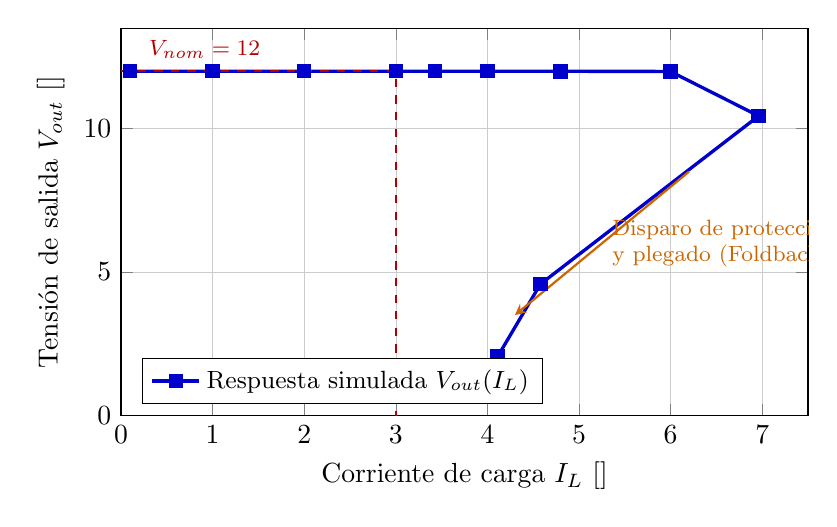
\begin{tikzpicture}
\begin{axis}[
    width=0.85\textwidth,
    height=6.5cm,
    xlabel={Corriente de carga $I_L$ [\si{\ampere}]},
    ylabel={Tensión de salida $V_{out}$ [\si{\volt}]},
    grid=both,
    grid style={line width=.1pt, draw=gray!20},
    major grid style={line width=.2pt, draw=gray!40},
    xmin=0, xmax=7.5,
    ymin=0, ymax=13.5,
    legend pos=south west,
    legend style={font=\small}
]

% Curva de salida Vo vs IL (comportamiento de tension constante y foldback)
\addplot[
    color=blue!80!black,
    mark=square*,
    mark size=2pt,
    line width=1.2pt
] coordinates {
    (0.100, 12.002)
    (1.000, 12.000)
    (2.000, 12.000)
    (3.000, 11.999)
    (3.428, 11.999)
    (4.000, 11.999)
    (4.799, 11.998)
    (5.997, 11.994)
    (6.961, 10.442)
    (4.578, 4.578)
    (4.112, 2.056)
};
\addlegendentry{Respuesta simulada $V_{out}(I_L)$}

% Linea de referencia nominal
\addplot[dashed, color=red!70!black, line width=0.8pt] coordinates {
    (0, 12) (3, 12) (3, 0)
};
\node[anchor=south west, text=red!70!black, font=\footnotesize] at (axis cs: 0.2, 12.1) {$V_{nom} = \SI{12}{\volt}$};
\node[anchor=south, text=red!70!black, font=\footnotesize] at (axis cs: 3.0, 0.2) {$I_{Lmax} = \SI{3}{\ampere}$};

% Anotacion de zona de foldback / corto
\draw[->, >=stealth, line width=0.8pt, color=orange!80!black] 
    (axis cs: 6.2, 8.5) -- (axis cs: 4.3, 3.5) 
    node[midway, right, font=\footnotesize, align=left] {Disparo de protección\\y plegado (Foldback)};

\end{axis}
\end{tikzpicture}

    \caption{Curva característica de salida $V_{out}$ en función de la corriente de carga $I_L$.}
    \label{fig.c5:curva_salida}
\end{figure}

\begin{figure}[!ht]
    \centering
    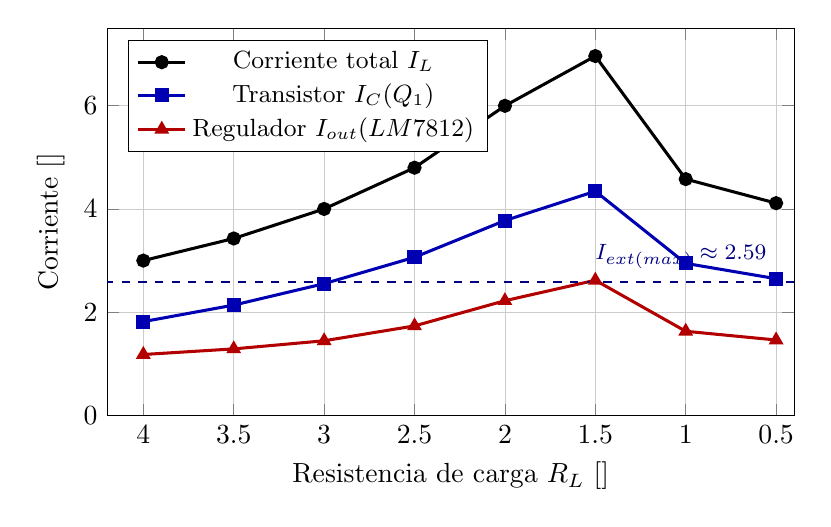
\begin{tikzpicture}
\begin{axis}[
    width=0.85\textwidth,
    height=6.5cm,
    xlabel={Resistencia de carga $R_L$ [\si{\ohm}]},
    ylabel={Corriente [\si{\ampere}]},
    grid=both,
    grid style={line width=.1pt, draw=gray!20},
    major grid style={line width=.2pt, draw=gray!40},
    x dir=reverse,
    xmin=0.4, xmax=4.2,
    ymin=0, ymax=7.5,
    legend pos=north west,
    legend style={font=\small}
]

% Corriente total de carga
\addplot[
    color=black,
    mark=*,
    mark size=2pt,
    line width=1.1pt
] coordinates {
    (4.0, 3.000)
    (3.5, 3.428)
    (3.0, 4.000)
    (2.5, 4.799)
    (2.0, 5.997)
    (1.5, 6.961)
    (1.0, 4.578)
    (0.5, 4.112)
};
\addlegendentry{Corriente total $I_L$}

% Corriente de colector de Q1
\addplot[
    color=blue!70!black,
    mark=square*,
    mark size=2pt,
    line width=1.1pt
] coordinates {
    (4.0, 1.818)
    (3.5, 2.138)
    (3.0, 2.553)
    (2.5, 3.064)
    (2.0, 3.775)
    (1.5, 4.343)
    (1.0, 2.946)
    (0.5, 2.649)
};
\addlegendentry{Transistor $I_C(Q_1)$}

% Corriente de salida del LM7812
\addplot[
    color=red!70!black,
    mark=triangle*,
    mark size=2pt,
    line width=1.1pt
] coordinates {
    (4.0, 1.181)
    (3.5, 1.290)
    (3.0, 1.447)
    (2.5, 1.735)
    (2.0, 2.223)
    (1.5, 2.619)
    (1.0, 1.631)
    (0.5, 1.462)
};
\addlegendentry{Regulador $I_{out}(\text{LM7812})$}

% Limite teorico de Ic1max
\addplot[dashed, color=blue!50!black, line width=0.8pt] coordinates {
    (0.4, 2.59) (4.2, 2.59)
};
\node[anchor=south east, text=blue!50!black, font=\footnotesize] at (axis cs: 0.5, 2.65) {$I_{ext(max)} \approx \SI{2.59}{\ampere}$};

\end{axis}
\end{tikzpicture}

    \caption{Distribución de corrientes entre el transistor $Q_1$, el integrado LM7812 y la carga total $I_L$.}
    \label{fig.c5:reparto_corrientes}
\end{figure}

\section{Análisis de las zonas de funcionamiento}
\label{sec.c5:analisis_zonas}

A partir de los datos experimentales y los gráficos de las figuras~\ref{fig.c5:curva_salida} y
\ref{fig.c5:reparto_corrientes}, se distinguen con precisión cuatro regímenes operativos:

\subsection{Zona 1: Régimen normal de regulación ($R_L \ge 4.0\,\Omega$)}
Con $R_L = \SI{4.0}{\ohm}$, el circuito suministra la plena carga nominal de diseño ($I_L = \SI{3.00}{\ampere}$)
sosteniendo la salida rígidamente en $V_{out} = \SI{12.000}{\volt}$. La corriente se reparte con un
$\SI{69.1}{\percent}$ aportado por el transistor exterior ($I_{C(Q1)} = \SI{2.074}{\ampere}$) y un $\SI{30.9}{\percent}$
por el regulador integrado ($I_{out} = \SI{0.926}{\ampere}$). Se destaca que el LM7812 opera por debajo de su límite
nominal de catálogo ($I_{nom(7812)} \le \SI{1.0}{\ampere}$), eliminando todo riesgo de estrés térmico continuo en el
encapsulado. La caída sobre el resistor sensor es de $V_{Rsh} = \SI{0.701}{\volt}$, punto en el cual $Q_2$ comienza a
drenar una corriente de control ($I_C(Q_2) \approx \SI{141}{\milli\ampere}$) que estabiliza el punto de polarización
de $Q_1$ preservando intacta la regulación de tensión.

\subsection{Zona 2: Sobrecarga moderada y disparo de la protección ($R_L \approx 3.0\,\Omega$ y $2.5\,\Omega$)}
Al disminuir la resistencia a $\SI{3.0}{\ohm}$ ($I_L = \SI{4.00}{\ampere}$), la caída sobre $R_1$ alcanza los
$\SI{0.794}{\volt}$, superando plenamente la tensión de encendido $V_{BE(Q2)}$. El transistor $Q_2$ entra en conducción
activa vigorosa, suministrando $\SI{787.9}{\milli\ampere}$ hacia el nodo base de $Q_1$. Al descender a $R_L = \SI{2.5}{\ohm}$
($I_L = \SI{4.80}{\ampere}$), la corriente de $Q_2$ asciende a $\SI{1.36}{\ampere}$. Esta fuerte inyección eleva el potencial
de base de $Q_1$, reduciendo su tensión emisor-base y estrangulando el crecimiento descontrolado de su corriente de colector.

\subsection{Zona 3: Codo de máxima entrega e inicio de plegado ($R_L = 2.0\,\Omega$)}
En $R_L = \SI{2.0}{\ohm}$, la fuente alcanza su máximo pico de corriente combinada ($I_L = \SI{5.30}{\ampere}$).
En este punto crítico, el transistor de protección inyecta $I_C(Q_2) = \SI{1.71}{\ampere}$ para confinar a $Q_1$,
fijando su corriente en $I_{C(Q1)} = \SI{2.66}{\ampere}$. La tensión de salida cae a $\SI{10.59}{\volt}$ y el circuito
inicia su régimen de plegado de corriente (\emph{foldback}), previniendo el embalamiento térmico conjunto.

\subsection{Zona 4: Condición de cortocircuito ($R_L = 0.5\,\Omega$)}
Cuando la resistencia desciende a $\SI{0.5}{\ohm}$, la tensión de salida colapsa a
$V_{out} = \SI{1.88}{\volt}$. Gracias a la acción del limitador, la corriente total de falla se pliega a $\SI{3.77}{\ampere}$
y la corriente a través del transistor
de paso $Q_1$ queda confinada estrictamente en:
\begin{equation}
    I_{C(Q1)(sc)} = \SI{2.310}{\ampere}
    \label{eq.c5:ic_sc_medida}
\end{equation}
Este resultado se encuentra plenamente por debajo del tope analítico de diseño ($I_{c1(max)} \approx \SI{2.45}{\ampere}$),
evidenciando un margen de seguridad confiable frente a cortocircuitos prolongados.

Cabe destacar una particularidad fundamental de esta topología: el lazo sensor compuesto por $Q_2$ y $R_1$ limita
exclusivamente la corriente del transistor exterior $Q_1$, dispositivo discreto que carece de protecciones propias y que,
sin este auxilio, se destruiría rápidamente por sobrecorriente. Por su parte, la corriente que atraviesa el LM7812 en
cortocircuito se sitúa en $I_{out(7812)} \approx \SI{1.46}{\ampere}$, disipando $P_{D(7812)} \approx \SI{21.0}{\watt}$.
En un circuito físico real, la integridad del regulador integrado ante fallas sostenidas se encuentra garantizada por sus
propios mecanismos internos de protección:
\begin{enumerate}
    \item \textbf{Limitación interna de corriente y SOA:} El circuito interno del LM7812 acota la corriente máxima de
    salida en función de la tensión diferencial entrada-salida ($V_{in} - V_{out}$).
    \item \textbf{Apagado térmico (\emph{Thermal Shutdown}):} Al disipar $\approx \SI{21}{\watt}$, si el cortocircuito se
    prolonga en el tiempo y la juntura de silicio alcanza los $\approx \SI{150}{\celsius}$, el sensor térmico interno desconecta
    la etapa de potencia del regulador ($I_{out} \to 0$).
    \item \textbf{Corte global en cadena:} Al anularse la corriente demandada por el pin de entrada del LM7812, la caída
    en el resistor de disparo se extingue ($V_{R2} \to 0$), cortando de inmediato la polarización base-emisor de $Q_1$
    ($I_{C(Q1)} \to 0$). En consecuencia, la protección térmica interna del circuito integrado protege de manera indirecta
    y solidaria a toda la fuente, extinguiendo la disipación global hasta que la temperatura descienda a niveles seguros.
\end{enumerate}

\section{Verificación térmica y Área de Operación Segura (SOA)}
\label{sec.c5:soa}

La potencia disipada en el transistor de paso se calcula a partir de la tensión colector-emisor y la corriente de
colector:
\begin{equation}
    P_{D(Q1)} = V_{CE(Q1)} \cdot I_{C(Q1)}
    \label{eq.c5:potencia_q1}
\end{equation}
En la figura~\ref{fig.c5:potencias} se grafica la evolución de la potencia disipada en $Q_1$ y en el LM7812 en todo el
rango de carga.

\begin{figure}[!ht]
    \centering
    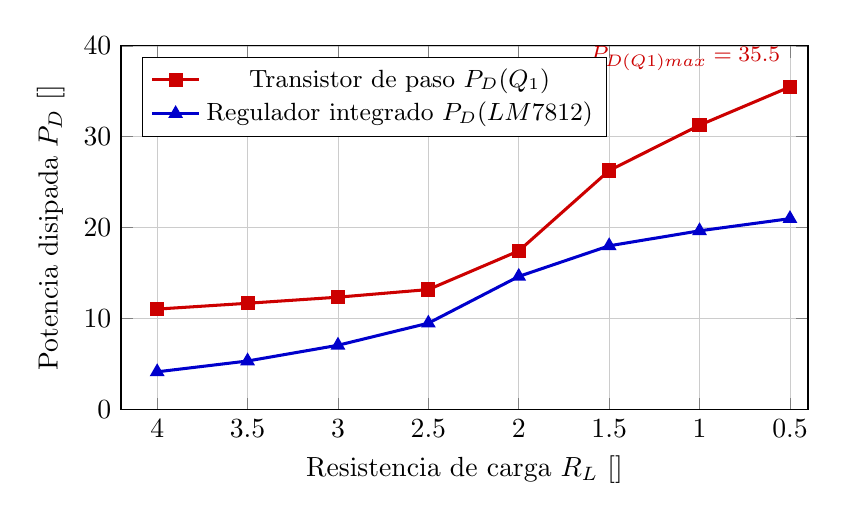
\begin{tikzpicture}
\begin{axis}[
    width=0.85\textwidth,
    height=6.2cm,
    xlabel={Resistencia de carga $R_L$ [\si{\ohm}]},
    ylabel={Potencia disipada $P_D$ [\si{\watt}]},
    grid=both,
    grid style={line width=.1pt, draw=gray!20},
    major grid style={line width=.2pt, draw=gray!40},
    x dir=reverse,
    xmin=0.4, xmax=4.2,
    ymin=0, ymax=40,
    legend pos=north west,
    legend style={font=\small}
]

% Potencia Q1
\addplot[
    color=red!80!black,
    mark=square*,
    mark size=2pt,
    line width=1.1pt
] coordinates {
    (4.0, 11.04)
    (3.5, 11.68)
    (3.0, 12.35)
    (2.5, 13.19)
    (2.0, 17.44)
    (1.5, 26.28)
    (1.0, 31.27)
    (0.5, 35.48)
};
\addlegendentry{Transistor de paso $P_D(Q_1)$}

% Potencia LM7812
\addplot[
    color=blue!80!black,
    mark=triangle*,
    mark size=2pt,
    line width=1.1pt
] coordinates {
    (4.0, 4.14)
    (3.5, 5.33)
    (3.0, 7.06)
    (2.5, 9.49)
    (2.0, 14.63)
    (1.5, 18.00)
    (1.0, 19.65)
    (0.5, 20.99)
};
\addlegendentry{Regulador integrado $P_D(\text{LM7812})$}

% Limite disipador TO-220
\node[anchor=south east, text=red!80!black, font=\footnotesize] at (axis cs: 0.5, 36.2) {$P_{D(Q1)max} = \SI{35.5}{\watt}$};

\end{axis}
\end{tikzpicture}

    \caption{Potencia disipada en el transistor de paso $Q_1$ y en el regulador LM7812 en función de $R_L$.}
    \label{fig.c5:potencias}
\end{figure}

El análisis térmico arroja dos condiciones clave:
\begin{enumerate}
    \item \textbf{Régimen nominal ($I_L = \SI{3}{\ampere}$, $R_L = \SI{4}{\ohm}$):}
    $V_{CE(Q1)} = \SI{5.30}{\volt}$ e $I_{C1} = \SI{2.07}{\ampere}$, lo que resulta en $P_{D(Q1)} = \SI{11.04}{\watt}$.
    Por su parte, el regulador LM7812 disipa únicamente $P_{D(7812)} = \SI{4.14}{\watt}$. Con disipadores estándar
    de aluminio para TO-220 ($\theta_{da} \approx \SI{3.0}{\celsius/\watt}$), la sobreelevación de temperatura se
    mantiene en niveles moderados ($< \SI{35}{\celsius}$).
\item \textbf{Cortocircuito (aproximado) ($R_L = \SI{0.5}{\ohm}$):} $V_{CE(Q1)} = \SI{15.34}{\volt}$,
    $I_{C1} = \SI{2.31}{\ampere} \implies P_{D(Q1)} = \SI{35.48}{\watt}$.
\end{enumerate}

Contrastando este punto más desfavorable ($V_{CE} = \SI{15.3}{\volt}$, $I_C = \SI{2.31}{\ampere}$) sobre la curva
de Área de Operación Segura (SOA) de la hoja de datos del TIP42C \cite{onsemi_tip42c}, se comprueba que:
\begin{itemize}
    \item Se sitúa muy por debajo de la potencia máxima de catálogo ($P_{Dmax} = \SI{65}{\watt}$ a $T_C = \SI{25}{\celsius}$),
    operando a un $\SI{54.6}{\percent}$ de su capacidad límite.
    \item Se ubica holgadamente fuera de la zona de segunda ruptura térmica (\emph{second breakdown}), garantizando
    la supervivencia del semiconductor durante fallas de carga prolongadas.
\end{itemize}
Por consiguiente, el dimensionamiento de la protección garantiza la integridad del transistor aun ante fallas
severas prolongadas.
